\documentclass[a4paper,12pt]{report}
\usepackage[top=1.25in, bottom=1.5in, left=0.9in, right=0.9in,headheight=20pt]{geometry}
\usepackage{pgfplots}
\pgfplotsset{compat=1.5}
\usepackage{tikz}
\usepackage{subcaption}
\usepgfplotslibrary{external}
\tikzset{>=latex}
\title{Title}
\date{}
\author{Ioannis Thyris}
% Start the documen
\begin{document}

\begin{figure}
\centering
\begin{subfigure}{\linewidth}
\centering
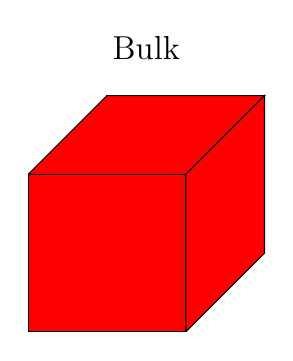
\begin{tikzpicture}
\node at (1.5,3.6) {\large{Bulk}};
\draw [fill=red] (1,1) rectangle (3,3);
\draw [fill=red] (0,0) rectangle (2,2);
\draw [fill=red] (0,2) -- (1,3) -- (3,3) -- (2,2) -- (0,2);
\draw [fill=red] (2,0) -- (2,2) -- (3,3) -- (3,1) -- (2,0);
\end{tikzpicture}
%
\hskip 10pt
%
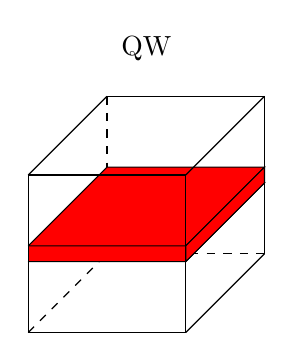
\begin{tikzpicture}
\node at (1.5,3.6) {QW};
\draw [dashed] (0,0) -- (1,1);
\draw [dashed] (1,3) -- (1,1);
\draw [dashed] (1,1) -- (3,1);
\draw [fill=red] (0,0.9)--(1,1.9)--(2,1.9)--(3,1.9)--(2,0.9)--(0,0.9);
\draw [fill=red] (0,0.9)--(0,1.1)--(2,1.1)--(2,0.9)--(0,0.9);
\draw [fill=red] (0,1.1)--(1,2.1)--(2,2.1)--(3,2.1)--(2,1.1)--(0,1.1);
\draw [fill=red] (2,0.9)--(2,1.1)--(3,2.1)--(3,1.9)--(2,0.9);
\draw (0,0) -- (2,0);
\draw (0,0) -- (0,2);
\draw (2,0) -- (2,2);
\draw (0,2) -- (2,2);
\draw (2,0) -- (3,1);
\draw (2,2) -- (3,3);
\draw (0,2) -- (1,3);
\draw (1,3) -- (3,3);
\draw (3,3) -- (3,1);
\end{tikzpicture}
%
\hskip 10pt
%
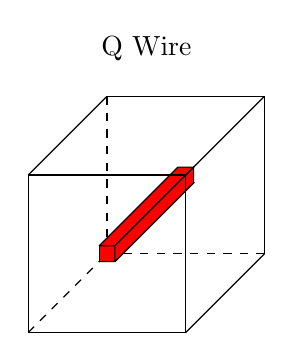
\begin{tikzpicture}
\node at (1.5,3.6) {Q Wire};
\draw [dashed] (0,0) -- (1,1);
\draw [dashed] (1,3) -- (1,1);
\draw [dashed] (1,1) -- (3,1);
\draw [fill=red] (0.9,0.9)--(1.9,1.9)--(2.1,1.9)--(1.1,0.9)--(0.9,0.9);
\draw [fill=red] (0.9,0.9)--(0.9,1.1)--(1.1,1.1)--(1.1,0.9)--(0.9,0.9);
\draw [fill=red] (0.9,1.1)--(1.9,2.1)--(2.1,2.1)--(1.1,1.1)--(0.9,1.1);
\draw [fill=red] (1.1,0.9)--(1.1,1.1)--(2.1,2.1)--(2.1,1.9)--(1.1,0.9);
\draw (0,0) -- (2,0);
\draw (0,0) -- (0,2);
\draw (2,0) -- (2,2);
\draw (0,2) -- (2,2);
\draw (2,0) -- (3,1);
\draw (2,2) -- (3,3);
\draw (0,2) -- (1,3);
\draw (1,3) -- (3,3);
\draw (3,3) -- (3,1);
\end{tikzpicture}
%
\hskip 10pt
%
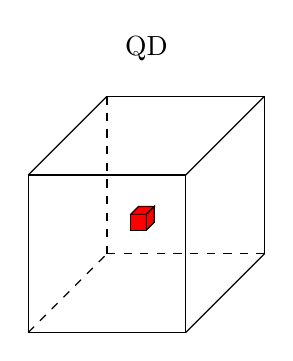
\begin{tikzpicture}
\node at (1.5,3.6) {QD};
\draw [dashed] (0,0) -- (1,1);
\draw [dashed] (1,3) -- (1,1);
\draw [dashed] (1,1) -- (3,1);
\draw [fill=red] (1.4,1.4) rectangle (1.6,1.6);
\draw [fill=red] (1.3,1.3) rectangle (1.5,1.5);
\draw [fill=red] (1.3,1.5)--(1.4,1.6)--(1.6,1.6)--(1.5,1.5)--(1.3,1.5);
\draw [fill=red] (1.5,1.3) -- (1.5,1.5) -- (1.6,1.6) -- (1.6,1.4) -- (1.5,1.3);
\draw (0,0) -- (2,0);
\draw (0,0) -- (0,2);
\draw (2,0) -- (2,2);
\draw (0,2) -- (2,2);
\draw (2,0) -- (3,1);
\draw (2,2) -- (3,3);
\draw (0,2) -- (1,3);
\draw (1,3) -- (3,3);
\draw (3,3) -- (3,1);
  \vspace*{10mm}
\end{tikzpicture}
\end{subfigure}
\par\bigskip
\begin{subfigure}{\linewidth}
\centering
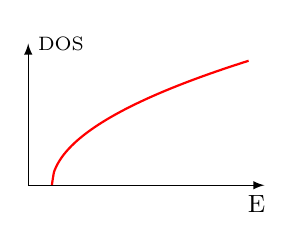
\begin{tikzpicture}
\draw[domain=0:2.5,smooth,samples=100,thick,red] plot (\x+0.3, {sqrt(\x)});
\draw [<->] (0,1.8) -- (0,0) -- (3,0);
\node [below] at (2.9,0) {\small{E}};
\node [right] at (0,1.8) {\scriptsize{DOS}};
\end{tikzpicture}
%
\hskip 10pt
%
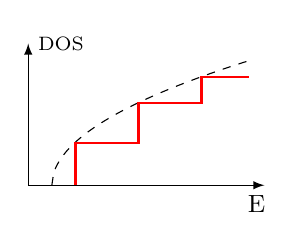
\begin{tikzpicture}
\draw[dashed,domain=0:2.5,smooth,samples=100] plot (\x+0.3, {sqrt(\x)});
\draw [thick,red] (0.6,0)--(0.6,0.54)--(1.4,0.54)--(1.4,1.04)--(2.2,1.04)--(2.2,1.37)--(2.8,1.37);
\draw [<->] (0,1.8) -- (0,0) -- (3,0);
\node [below] at (2.9,0) {\small{E}};
\node [right] at (0,1.8) {\scriptsize{DOS}};
\end{tikzpicture}
%
\hskip 10pt
%
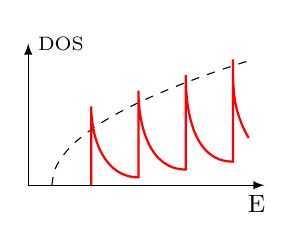
\begin{tikzpicture}
\draw[dashed,domain=0:2.5,smooth,samples=100] plot (\x+0.3, {sqrt(\x)});
\draw [<->] (0,1.8) -- (0,0) -- (3,0);
\draw [thick,red] (0.8,0)--(0.8,1) to [out=-90,in=180] (1.4,0.1)--(1.4,1.2) to [out=-90,in=180] (2,0.2)--(2,1.4) to [out=-90,in=180]  (2.6,0.3)--(2.6,1.6) to [out=-90,in=120] (2.8,0.6);
\node [below] at (2.9,0) {\small{E}};
\node [right] at (0,1.8) {\scriptsize{DOS}};
\end{tikzpicture}
%
\hskip 10pt
%
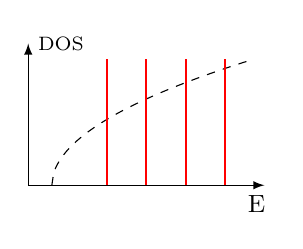
\begin{tikzpicture}
\draw[dashed,domain=0:2.5,smooth,samples=100] plot (\x+0.3, {sqrt(\x)});
\draw [<->] (0,1.8) -- (0,0) -- (3,0);
\draw [thick,red] (1,0)--(1,1.6);
\draw [thick,red] (1.5,0)--(1.5,1.6);
\draw [thick,red] (2,0)--(2,1.6);
\draw [thick,red] (2.5,0)--(2.5,1.6);
\node [below] at (2.9,0) {\small{E}};
\node [right] at (0,1.8) {\scriptsize{DOS}};
\end{tikzpicture}
\end{subfigure}
\caption{\small{Structures of reduced dimensionality and their corresponding density of states, compared to the bulk material.}}
\label{fig:dos}
\end{figure}

\end{document}
